%% -*- coding: utf-8 -*-
\documentclass[12pt,a4paper]{scrartcl} 
\usepackage[utf8]{inputenc}
\usepackage[english,russian]{babel}
\usepackage{indentfirst}
\usepackage{misccorr}
\usepackage{graphicx}
\usepackage{amsmath}
\usepackage{float}
\usepackage{ dsfont }

\usepackage{xcolor}
\usepackage{hyperref}
\hypersetup{colorlinks,
  pdftitle={The title of your document},
  pdfauthor={Your name},
  allcolors=[RGB]{000 000 000}}

\begin{document}
\begin{titlepage}
  \begin{center}

    Санкт-Петербургский политехнический университет Петра Великого

    \vspace{0.25cm}
    
    Институт прикладной математики и механики
    
    Кафедра «Прикладная математика»
    \vfill

	\vspace{0.25cm}
	    Отчёт\\
	по лабораторной работе №2\\
	по дисциплине\\
	«Вычислительные комплексы»

  \bigskip

\end{center}
\vfill

\newlength{\ML}
\settowidth{\ML}{«\underline{\hspace{0.7cm}}» \underline{\hspace{2cm}}}
\hfill\begin{minipage}{0.4\textwidth}
  Выполнил студент\\ В.\,А.~Рыженко\\
\end{minipage}%
\bigskip

\hfill\begin{minipage}{0.4\textwidth}
  Проверил:\\
к.ф.-м.н., доцент\\
Баженов Александр Николаевич\\
\end{minipage}%
\vfill

\begin{center}
  Санкт-Петербург, 2020 г.
\end{center}
\end{titlepage}

\tableofcontents
%\listoffigures
\newpage


\section{Постановка задачи}

Для демонстрации интервальной глобальной минимизации использовать функцию:
\begin{equation}
    function [Z, WorkList] = globopt0(X).
\end{equation}
Она возвращает значение глобального экстремума Z и рабочий список WorkList. Работа алгоритма построена на последовательном сужении множества, на котором строится оптимум.

\subsection{Задача 1}
Рассмотреть пример из лекционного материала. Построить рабочий список, построить график сужения интервала.


\subsection{Задача 2}
Взять пример с \cite{test_opt} и изучить сходимость.

\section {Теория}


\subsection{Алгоритм GlobOpt}
	Алгоритм для глобальной минимизации функции GlobOpt оперирует с рабочим списком $\zeta$, в котором будут храниться все брусы, получающиеся в результате дробления исходного бруса области
    определения на более мелкие подбрусы.
    \newline
    Одновременно с самими
    подбрусами будем хранить в рабочем списке и нижние оценки областей значений целевой функции по этим подбрусам, так что элементами списка $\zeta$ будут записи-пары вида:
    \begin{equation}
        \zeta: (Y, y), \text{где} Y  \subseteq X, y = f(Y).
    \end{equation}

	Первоначально в рабочий список помещается одна запись
	
	\begin{equation}
		(X, f(X)),
	\end{equation}

	Далее каждый шаг алгоритма состоит в извлечении из этого списка
    бруса, который обеспечивает рекордную (т. е. наименьшую) на данный
    момент оценку минимума снизу, его дроблении на более мелкие
    подбрусы, оценивании на них целевой функции, занесении результатов
    обратно в рабочий список.
    
    \subsection{Функция Розенброка}
	Имеет вид:
	\begin{equation}
	    f_{R} = 100 \cdot ({x_1}^2 - x_2)^2 - (x_1 - 1)^2
	    \label{rozen}
	\end{equation}
	Минимум функции достигается при значении аргумента x = (1, 1) и равен 0.

	\begin{figure}[H]
        \centering
        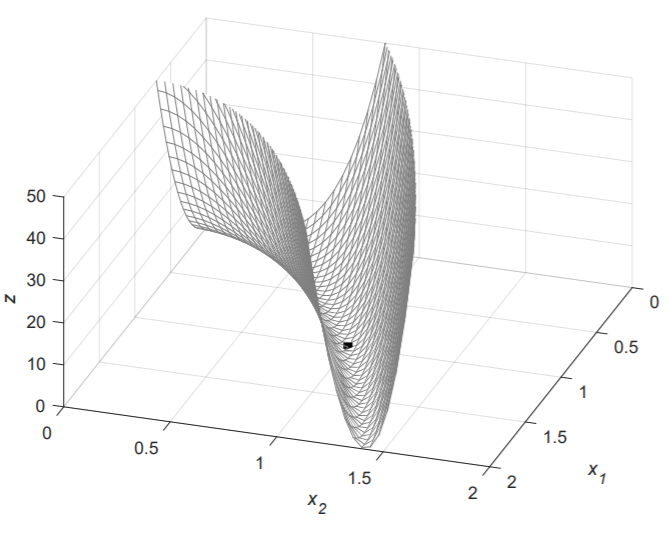
\includegraphics[width=7cm,height=7cm]{fig/rosen_func.png}
        \caption{Функция Розенброка}
        \label{fig:rossen}
    	\end{figure}

	\subsection{Schaffer function N. 2}
	Имеет вид:
	\begin{equation}
	    f_{C} = 0.5 + \frac{\sin^2(x^2-y^2) - 0.5}{[1 + 0.001(x^2 + y^2)]^2}
	    \label{schaffer}
	\end{equation}
	Минимум функции достигается при значении аргумента x = (-100, 100) и равен 0.
    \begin{figure}[H]
        \centering
        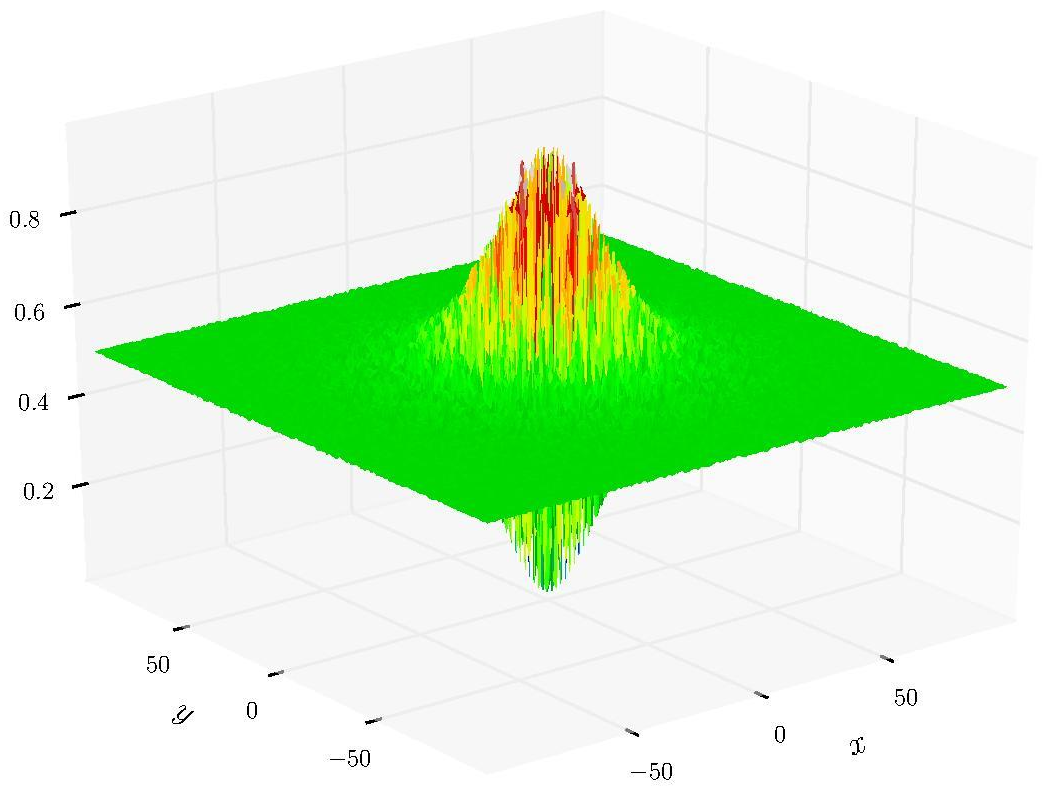
\includegraphics[width=10cm,height=8cm]{fig/schaf_func.png}
        \caption{Schaffer function N. 2}
        \label{fig:schaffer}
    \end{figure}


\section {Реализация}
Лабораторная работа выполнена с помощью встроенных средств языка программирования Matlab, оптимизатор globopt0 и библиотеки для интервальной арифметики IntLab. Исходный код лабораторной работы приведён в приложении.

\section {Результаты}

\subsection{Задача 1}
Рабочий список автоматически генерируется и реализован в качестве массива, содержащий в себе значения бруса и целевой функции.

Далее представлен график зависимости размера области от количества итерации. Размер области считается как сумма диаметров интервальных компонент брусов. \\
Задаем брус, на котором ищем решение, как
$X = [-30, 30] \times [-30, 30]$. \\
\begin{figure}[H]
    \centering
    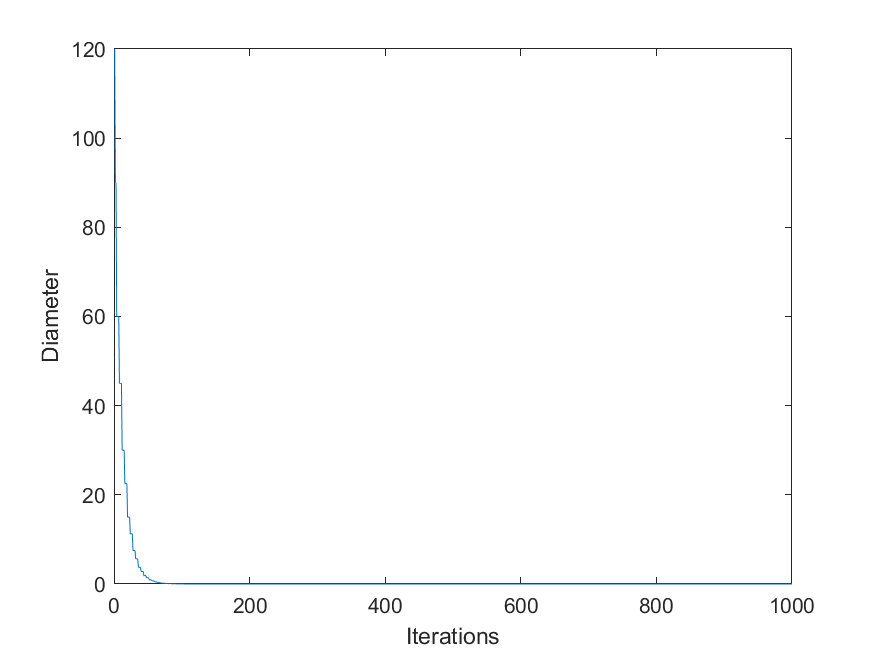
\includegraphics[width=10cm, height=8cm]{fig/rosenbrock.png}
    \caption{Сужение бруса для функции Растригина}
    \label{fig:rast}
\end{figure}
 
\subsection{Задача 2}
Рассмотрим оптимизацию функцию (\ref{schaffer}).\\
Задаем брус, на котором ищем решение, как
$X = [-50, 50] \times [-50, 50]$. \\
Исследуем зависимость значения функции от количества итераций.
\begin{table}[H]
    \centering
    \begin{tabular}{| c | c |}
        \hline
         Число итераций & $min(f_{C}(x, y))$ \\ \hline
         5 & 0.3107 \\ \hline
         10 & 0.1260 \\ \hline
         20 & 0.0369 \\ \hline
         30 & 0.0096 \\ \hline
	   40 & 0.0024 \\ \hline
	   100 & 3.7252e-08 \\ \hline
         200 & 2.1649e-15 \\ \hline
    \end{tabular}
    \label{tab:tav}
\end{table}
Из (\ref{tab:tav}) видно, что вычисленное значение довольно быстро приближается к истинному.\\

Далее рассмотрим зависимость абсолютной погрешности $|x_{*} - x_{n}|$ от количества итераций. Где $x_{n}$ найденное значение на данной итерации и $x_{*}$ истинное значение минимума.
\begin{figure}[H]
    \centering
    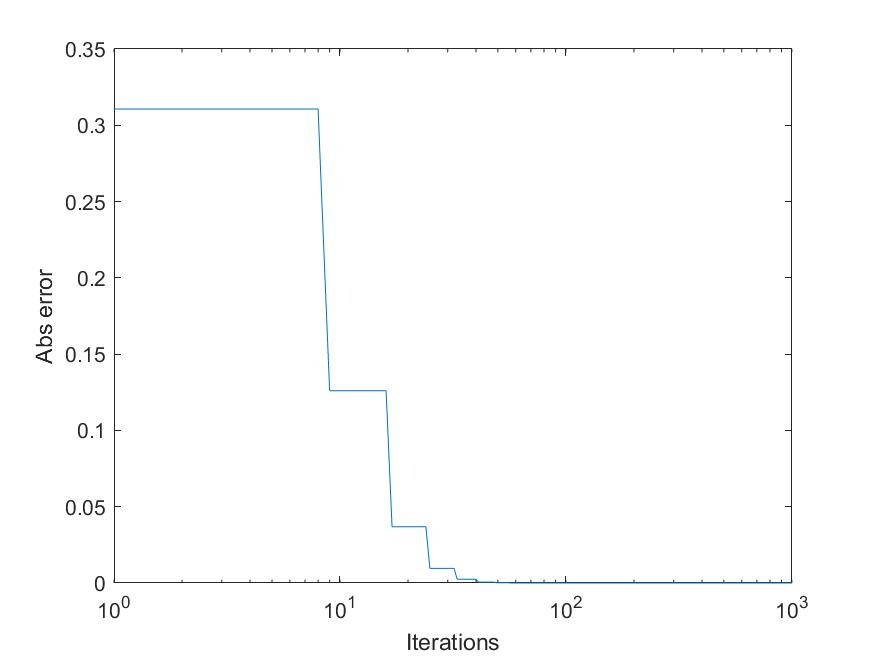
\includegraphics[width=10cm, height=8cm]{fig/convergence.png}
\end{figure}

Из графика видно, что метод достаточно хорошо сходится для данной функции. Погрешность порядка $10^{-3}$ достигается уже на 41 итерации.

\section{Приложения}
Репозиторий на GitHub с релизацией: \href{https://github.com/WiillyWonka/Intervals}{github.com}.
\end{document}

\end{document}
